
%
% state - vis
%

\section{Visual mapping}
\label{state-vis}

N\"{o}llenburg~\cite{noellenburg11geovis} names three ``Driving forces in geovisualization'': The advent of high speed parallel processing and technology advances in computer graphics, today allows us to grasp enormous amounts of information. Besides the advances in graphics and display technologies, the second main driving force in geographic visualization is the increasing amount of geospatial data being collected and available. Finally, the third force is the \textit{rise of the Internet}, which significantly pushes web mapping and contributes to geovisualization technologies.

As a logical consequence of broader audiences having access to geospatial visualizations using the Internet, it appears that there is a shift from technology-driven visualization towards more human-centered approaches. Interactive and highly dynamic interfaces have helped the map evolve from its traditional role as a presentational device towards exploring geospatial data~\cite{noellenburg11geovis, vislecture}.

In chapter \ref{chapter:foundations-vis}, foundations of visualization, visual variables and data exploration techniques, as well as the concept of clutter reduction have been introduced. In the following, existing visualization techniques for representing clustered data on maps will be discussed. In a first step, visualization concepts on the map level will be investigated. Later, approaches for visualizing individual clusters are added. An evaluation summarizes the discussed technologies. 

\subsection{Map visualization types for clustering}
\label{chapter:map-vis}

There exists a variety of map types, serving different purposes like standard \textit{geographic maps}, \textit{cartograms}, \textit{geologic maps}, \textit{linguistic maps} or \textit{weather maps}. Some of these use distortion, for example the cartogram can be used to map the area of each country to the size of population. In this section, we try to identify those map types which are appropriate for visualizing clustered data~\cite{noellenburg11geovis, wiki:map-types}:

\begin{itemize}

\item \textbf{Geographic map with markers}. The default way of representing data is a standard 2-dimensional map with markers on top of it. Each marker represents a data point, or in the case of clustering, a cluster.

\parbox [h]{0.4\textwidth}{
    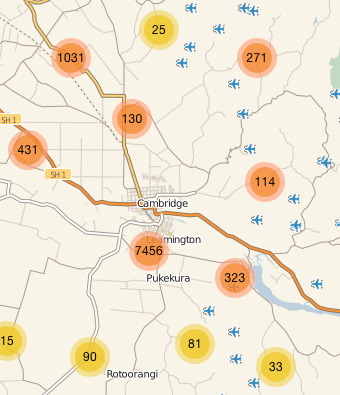
\includegraphics [width=\linewidth]{figures/map_types_normal_leaflet.png}
    \captionof {figure}{Leaflet map}
    \label{fig:map-type-standard-leaflet}
}
\hfill
\hspace{0.5cm}
\parbox [h]{0.4\textwidth }{
    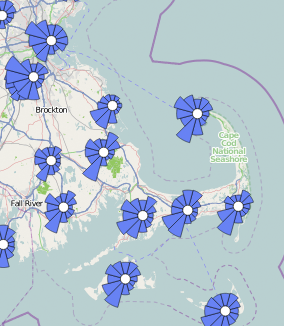
\includegraphics [width=\linewidth]{figures/map_types_standard_wind.png}
    \captionof {figure}{Wind history map}
    \label{fig:map-type-standard-wind}
}

\begin{itemize}

\item Figure \ref{fig:map-type-standard-leaflet} depicts an example\footnote{Leaflet.clustermarker example map from \url{http://leaflet.github.io/Leaflet.markercluster/example/marker-clustering-realworld.10000.html}} of the Leaflet.markercluster library. Clustered results are displayed using markers of the same size. The amount of items within a cluster is indicated using text within the markers and by using a ``hot-to-cold'' color ramp~\cite{web:color-ramp}. 

\item Figure \ref{fig:map-type-standard-wind} shows a similar example, in this case a Wind history map\footnote{Wind history map \url{http://windhistory.com/map.html}} with markers for every wind measurement point. An advanced visualization technique is used for visualizing the amount of wind per cardinal direction as \textit{polar area diagram}.

\end {itemize}

These two variations of standard maps shall indicate the potential of using advanced visualization techniques for displaying cluster items. Further ways for cluster visualization will be discussed in chapter \ref{chapter:cluster-vis}.

\item \textbf{Geographic Heat map}

Heat maps use colored, two-dimensional areas to express the value of each data entity on the map. \textit{Choropleth maps} are the most common heat maps, which are often used for analysis of geographic and statistical data. 

\parbox [h]{0.4\textwidth}{
    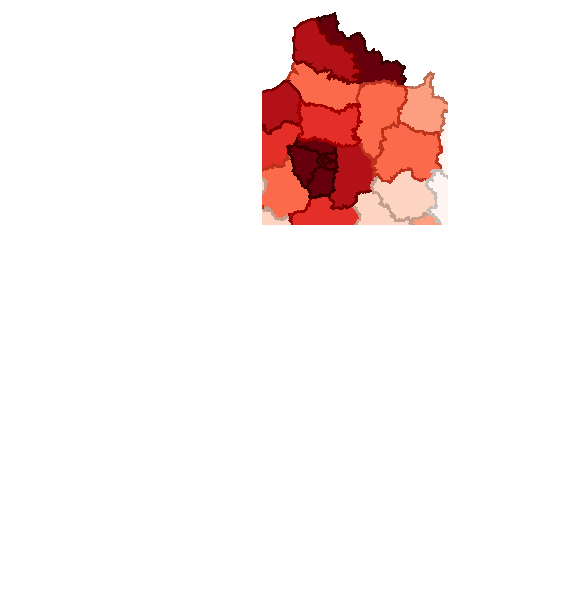
\includegraphics [width=\linewidth]{figures/map_types_choropleth.pdf}
    \captionof {figure}{Choropleth map\protect\footnotemark}
    \label{fig:map-type-choropleth}
}\footnotetext{Choropleth map example from Kartograph \url{http://kartograph.org/showcase/choropleth/}}
\hfill
\hspace{0.5cm}
\parbox [h]{0.4\textwidth}{
    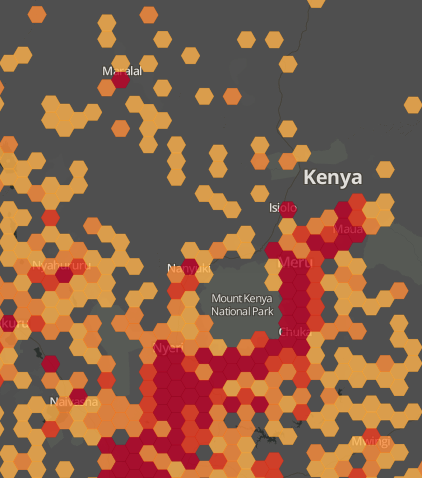
\includegraphics [width=\linewidth]{figures/map_types_heatmap.png}
    \captionof {figure}{Heat map\protect\footnotemark}
    \label{fig:map-type-binning}
}\footnotetext{Heat map that uses binning \url{http://mapbox.com/blog/binning-alternative-point-maps/}}


\begin{itemize}

\item Figure \ref{fig:map-type-choropleth} visualizes an example choropleth map that shows population data for each of the departments of metropolean France. Color coding is used to indicate densely populated regions with heavier red tones.

\item Figure \ref{fig:map-type-binning} presents another example that uses \textit{binning} for creating a hexagonal tessellation of the surface in order to visualize clustered results. 

\end {itemize}

A problem with heat maps is that they require a non-overlapping tessellation of the surface to provide the areas for visualization. As the binning example indicates, such a tessellation can be done programmatically. Heat maps therefore can also be used for visualizating arbitrary clustered data without a need to calculate the exact boundaries of clusters. Another variation of heat maps is the \textit{prism map}, which adds extrusion of areas as a third dimension~\cite{ladenhauf12dia, Delort10vis}. A publication on the evaluation of color schemes in choropleth maps can be found in~\cite{MacEachrenMort}. 


\item \textbf{Dot grid maps}

Dot grid maps are based on the suggestion by Jaques Bertin~\cite{bertin67graphics, bertin83graphics} to use graduated sizes in a regular pattern as an alternative to chloropeth maps. The advantage is that the map creator doesn't have to choose between quantity or density of a distribution value, because the dot grid map shows both a the same time. The user can understand the data distribution on a finer level of granularity, as opposed to where the chloropeth map usually creates larger areas of aggregated information~\cite{web:dot-grid}.

Figure \ref{fig:map-type-dotgrid} is an alternative version of the France map from figure \ref{fig:map-type-choropleth}, visualized as a dot grid map.


\item \textbf{Voronoi map}

The Voronoi tessellation is a space partitioning technique. From a set of points it produces a Voronoi polygon for each point, such that the area covered is closest to that point in comparison to all other points. Jean-Yves Delort describes a technique that uses Voronoi polygons for ``Vizualizing Large Spatial Datasets in Interactive Maps''~\cite{Delort10vis}. It uses a hierarchical clustering technique to choose a subset of points per zoom level for proper visualization. Still, the effectiveness of this approach is questionable, as the scalability analysis of the studies shows that the technique can efficiently be used for datasets of up to 1000 items.

Figure \ref{fig:map-type-voronoi} shows an exemplary voronoi map that displays all U.S. airports as of 2008. Besides the shown visualization, for Voronoi maps apply the same visualization possibilities as for cloropeth maps.

\parbox [h]{0.4\textwidth }{
    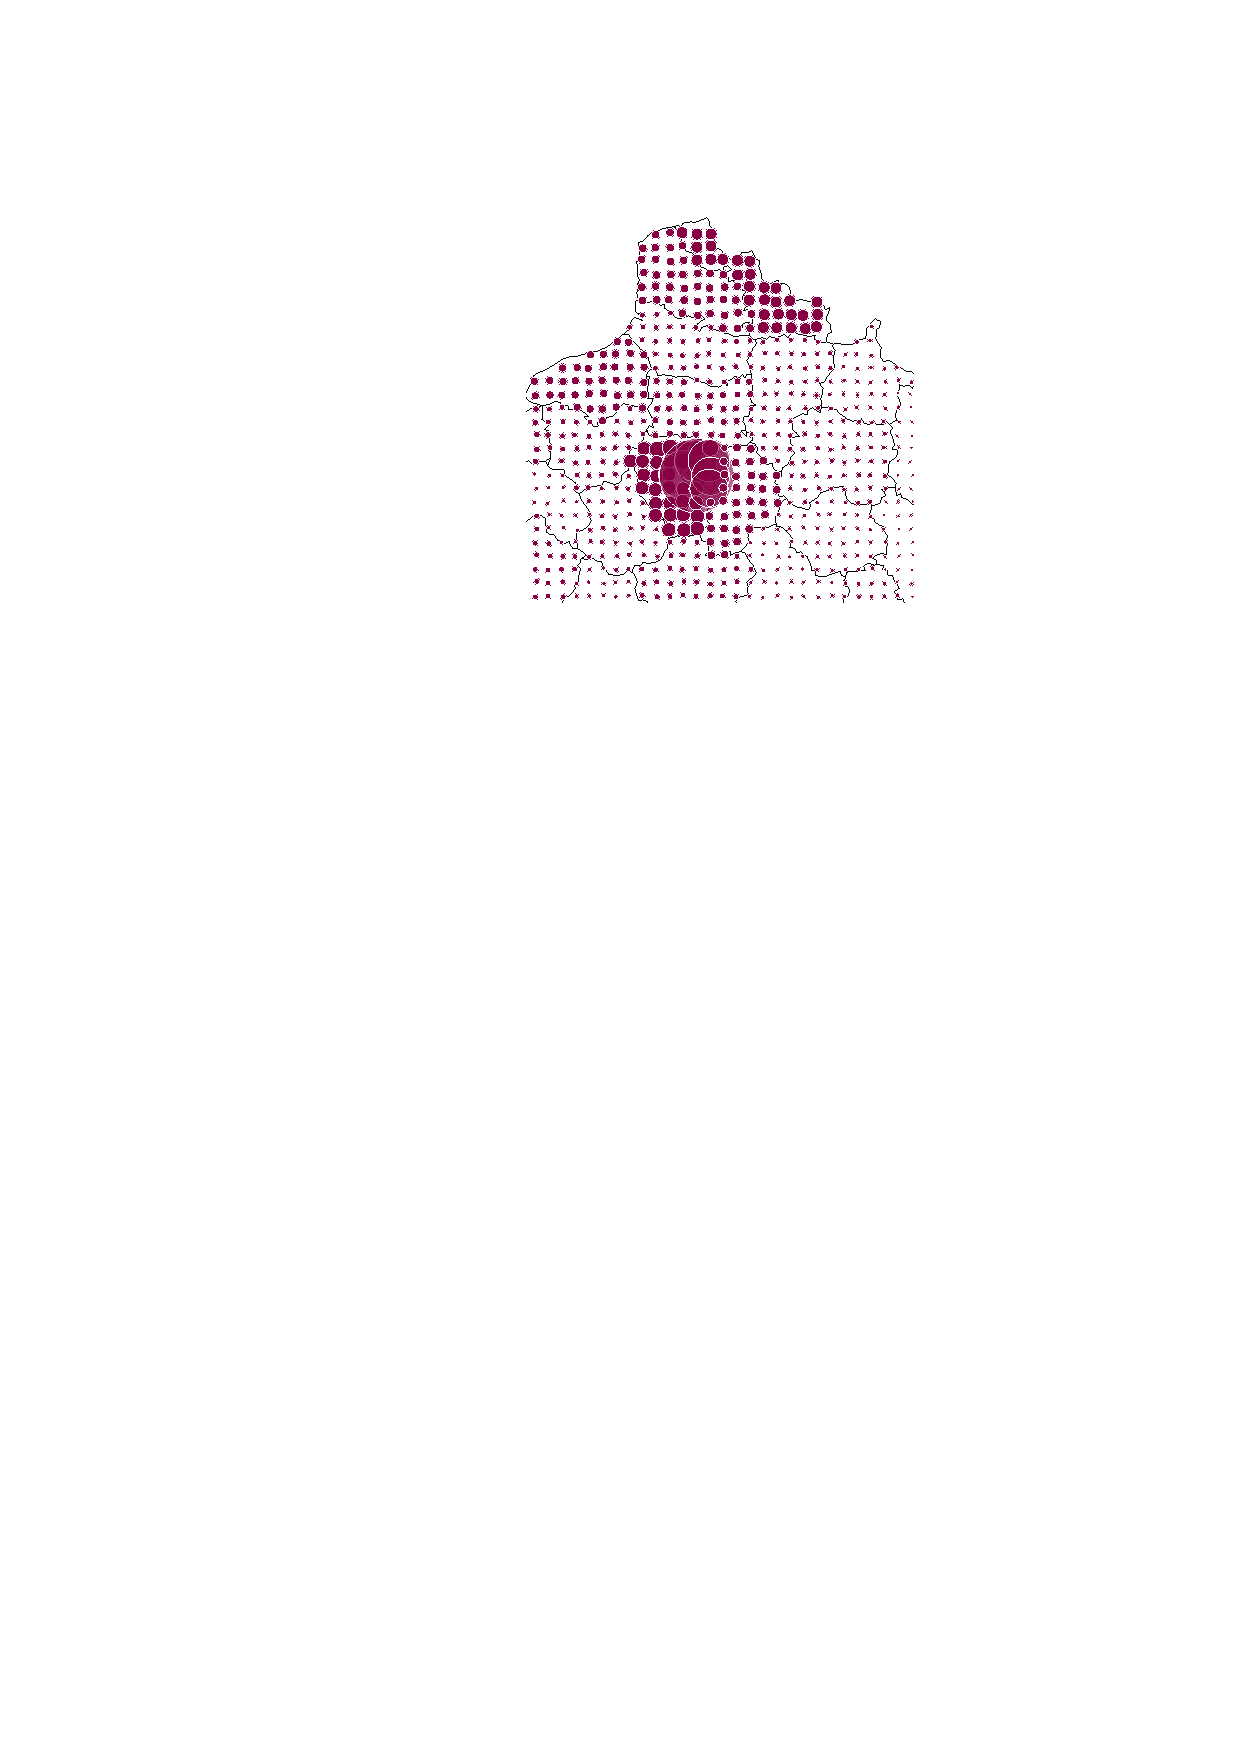
\includegraphics [width=\linewidth]{figures/map_types_dot_grid.pdf}
    \captionof {figure}{Dot Grid map\protect\footnotemark}
    \label{fig:map-type-dotgrid}
}\footnotetext{Dot Grid map example from Kartograph \url{http://kartograph.org/showcase/dotgrid/}}
\hfill
\hspace{0.5cm}
\parbox [h]{0.4\textwidth }{
    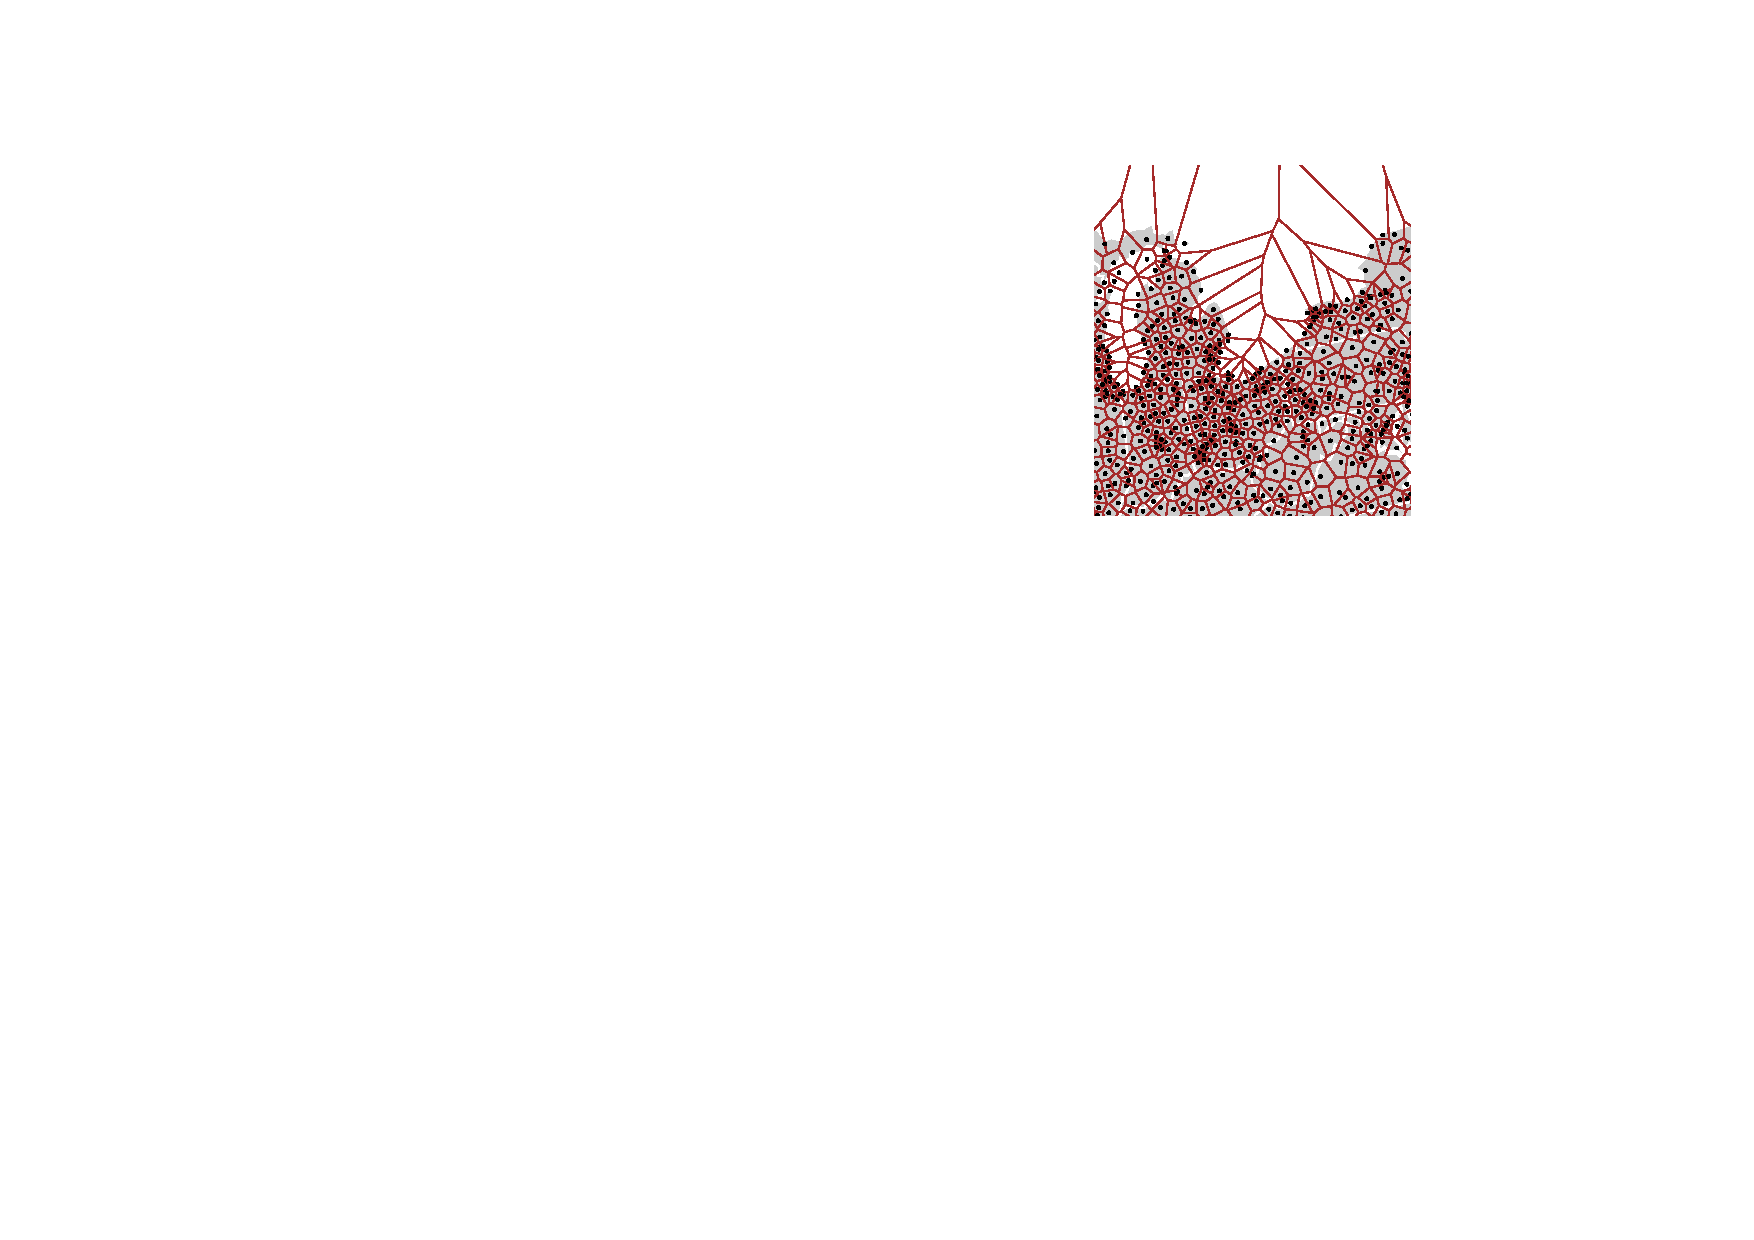
\includegraphics [width=\linewidth]{figures/map_types_voronoi.pdf}
    \captionof {figure}{Voronoi map\protect\footnotemark}
    \label{fig:map-type-voronoi}
}\footnotetext{Voronoi map example \url{http://mbostock.github.io/d3/talk/20111116/airports-all.html}}

\end{itemize}

\textit{Self-organizing maps} (SOM) can also be used to visualize clusters of data. But instead of displaying data on a geographic map, self-organizing maps create their own virtual space in order to represent information~\cite{noellenburg11geovis}.  


\subsection{Cluster visualization techniques for maps}
\label{chapter:cluster-vis}

The previous chapter has shown different kinds of map visualization techniques appropriate for displaying clustered data. In the end, each visualization will show (clustered) items on a map as visual objects with attributes like a particular shape or coloring. As clusters contain aggregated information, an important task is to find the right way for visualizing the cluster items themselves. From the examples provided so far, we have seen variations in size, shape and color which expose information on the cluster items being visualized on the map. In the following, multivariate data visualization techniques will be evaluated for visualizing cluster items on a map.

In chapter \ref{vis-data-techniques}, a classification of visualization techniques by data type and interaction technique has been presented. Ke-Bing Zhang~\cite{zhang07thesis} has written about ``Visual Cluster Analysis in Data Mining'', where he list an extensive list of multivariate data visualization techniques. Potentially, any such visualization technique can be used, but the frame of the map puts constraints in terms of space on the representation of individual items. \textit{Iconic displays} are a simple way to visualize data, which also prevents clutter. \textit{Dense Pixel} displays and \textit{geometric visualizations} like charts can be used to encode more complex information.

\begin{itemize}

\item \textbf{Icon-based, Glyphs}

Matthew O Ward \cite{ward02glyphs} defines \textit{glyphs} as ``graphical entities that convey one or more data values via attributes such as shape, size, color, and position''. While the work of Otto Neurath on \textit{ISOTYPE}~\cite{neurath} (1930s) can be seen as fundamental for \textit{pictorial statistics}, the best-known literature reference to glyphs is ``Chernoff faces''~\cite{chernoff73}. As (e) figure \ref{fig:glyphs-ward} indicates, data is encoded into properties of the face icon, such as shape of nose, mouth, eyes. Other fundamental glyph-based techniques include \textit{stick figures}~\cite{stickfigures}, \textit{color icons}~\cite{coloricons}, \textit{Hyperbox}~\cite{hyperbox} and \textit{shape coding}~\cite{shapecoding}. Figure \ref{fig:glyphs-ward} extends this list by showing examples of glyphs that Ward collected for his taxonomy of glyphs placement strategies~\cite{ward02glyphs}.

\begin{figure}[h]
  \begin{center}
    \hspace*{-1cm}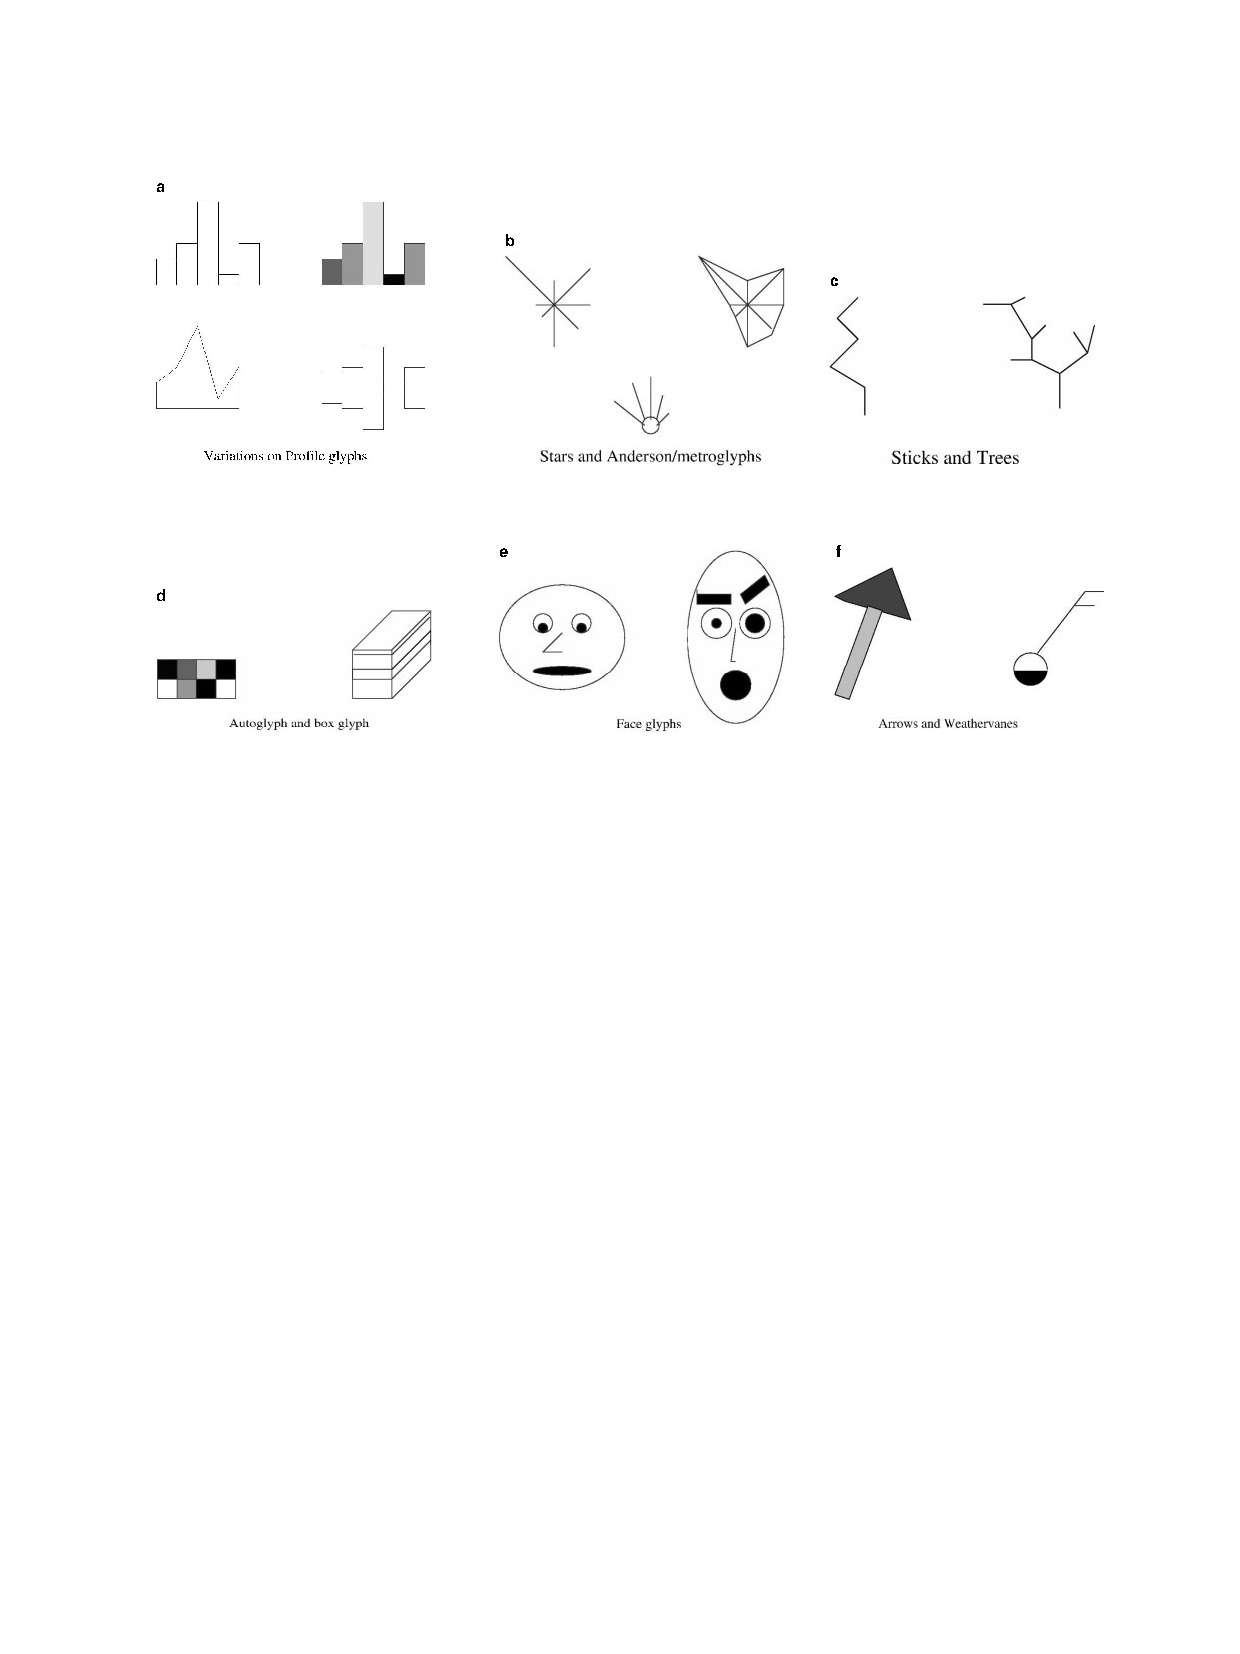
\includegraphics[width=1.2\textwidth]{figures/glyphs.pdf}
    \caption{Examples of glyphs. Top row: (a) variations on profiles; (b) stars/metroglyphs; and (c) stick figures and trees.
Bottom row: (d) autoglyphs and boxes; (e) faces; and (f) arrows and weathervanes.~\cite{ward02glyphs}.}
    \label{fig:glyphs-ward}
  \end{center}
\end{figure}

Some glyph types have been created to identify clusters or similarities by plotting them side-by-side on a 2-dimensional plane, a technique which is referred to as \textit{mosaic-based rendering}. \textit{Stick figures} and \textit{mosaic metaphors} are examples in that field~\cite{stickfigures, nocke05mosaic}. One the other hand, reducing visual clutter as explained in chapter \ref{clutter-reduction} also matters for glyphs, especially when putting them on a map. A trade-off between information-richness vs. simplicity and clarity has to be made. As Zhang writes, ``with the amount of data increasing, the user hardly makes any sense of most properties of data intuitively, this is because the user cannot focus on the details of each icon when the data scale is very large''~\cite{zhang07thesis}. We can compare this to the map use cube presented in chapter \ref{chapter:foundations-vis}: more complex glyph types seem to be better suited for scientific purposes which can be related to private uses, while simpler glyph types seem more appropriate for presenting data to a public audience.

Examples for uses of simple icons and glyph types for clustered data on maps can be found in JavaScript mapping libraries as seen in chapter \ref{chapter:client-side-web-mapping}. These are usually based on a simple icon or geometric shape like a circle or marker and use color coding and size variations as indicators for underlying information. Further examples are scaled data values and scaled dots \cite{web:scaled-data-value}, as well as the proportional symbol map \cite{vislecture}. In contrast to those presented so far, figure \ref{fig:glyphs-zame} visualizes eight simple glyphs~\cite{ElmqvistDGHF08}.

\begin{figure}[h]
  \begin{center}
    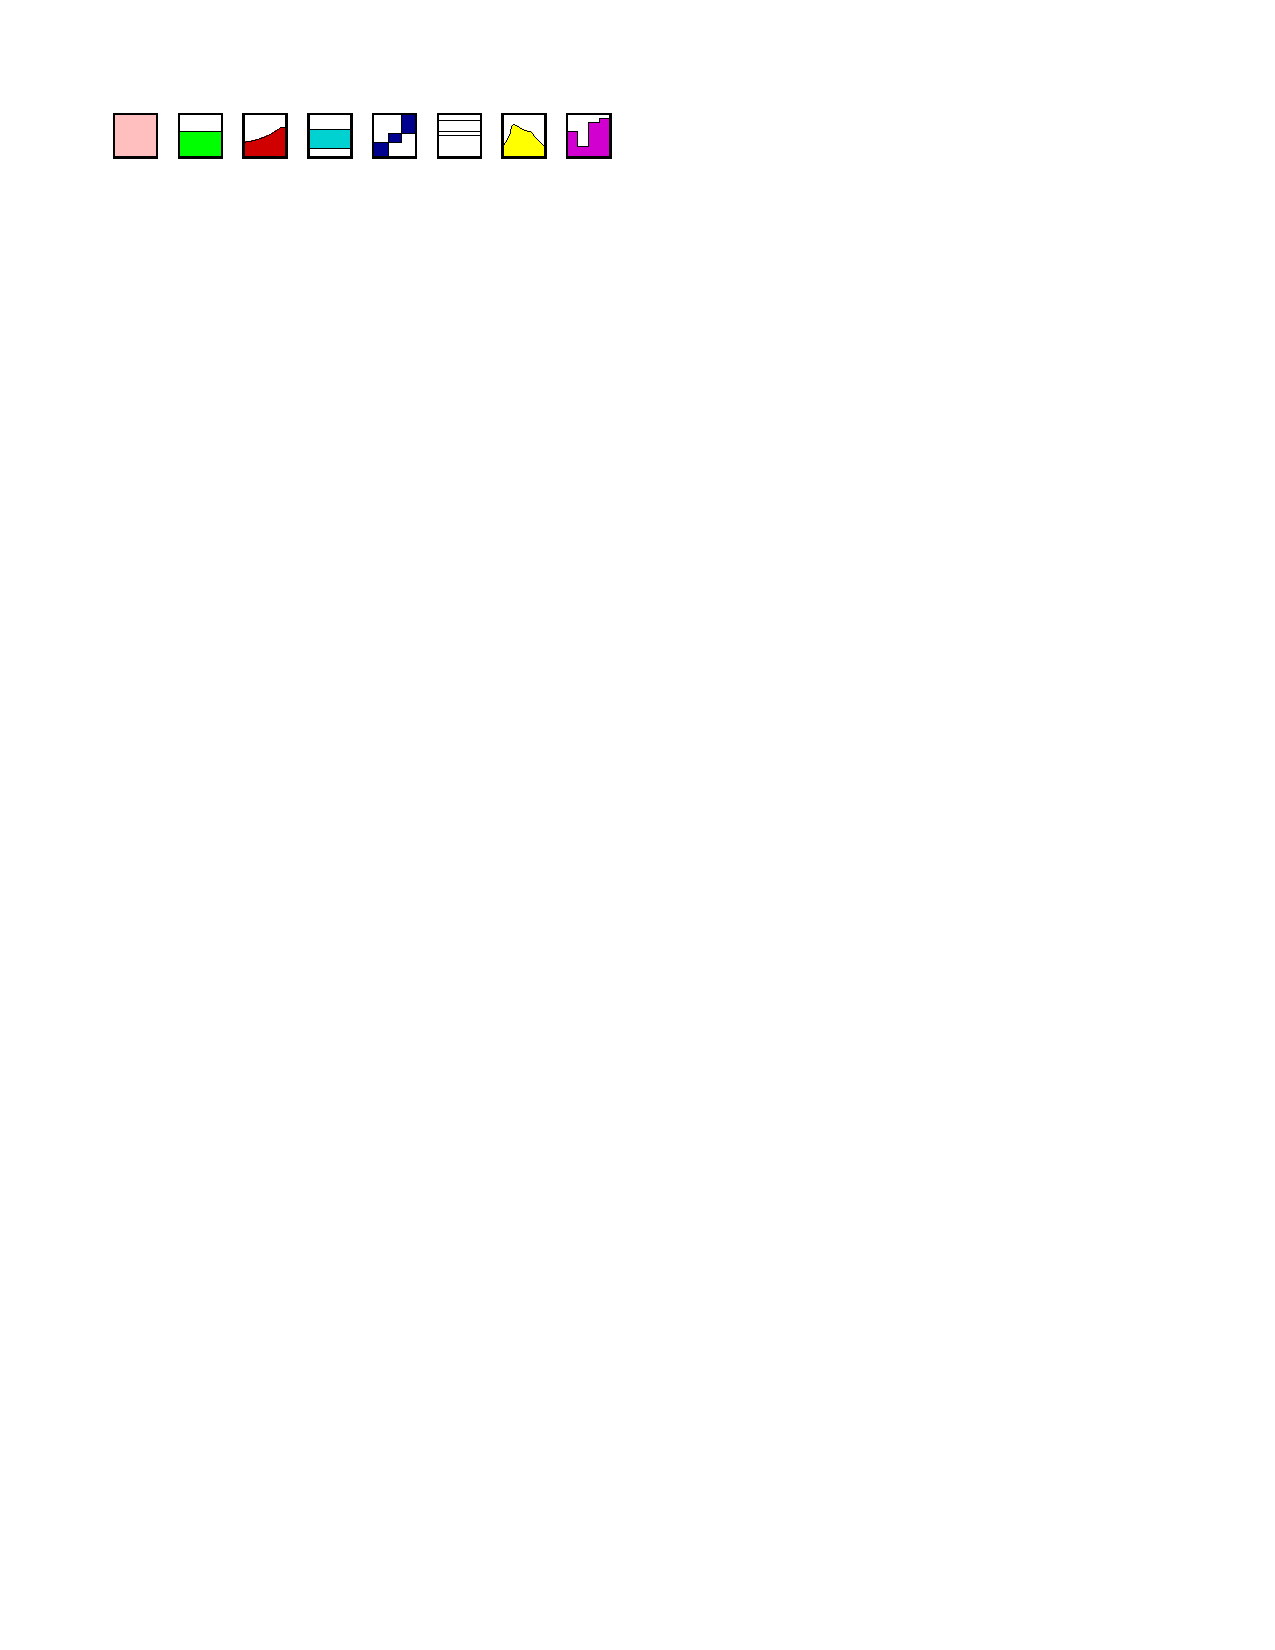
\includegraphics[width=0.65\textwidth]{figures/glyphs_zame.pdf}
    \caption{Eight different glyphs for aggregated edges (color shade,
average, min/max histogram, min/max range, min/max tribox, Tukey
box, smooth histogram, step histogram)~\cite{ElmqvistDGHF08}.}
    \label{fig:glyphs-zame}
  \end{center}
\end{figure}


\item \textbf{Pixel-oriented}

Pixel-oriented techniques display the most possible information at a time by mapping each attribute value of data to a single, colored pixel. Color mapping approaches such as \textit{linear variation of brightness}, \textit{maximum variation of hue} and \textit{constant maximum saturation} are used to color pixels which are arranged within limited space. By providing an overview of large amounts of data, pixel-oriented display techniques are suitable for a variety of data mining tasks in combination with large databases~\cite{zhang07thesis}.

The first pixel-oriented technique was presented by Keim~\cite{keim94pixel} as part of the \textit{VisDB system}. Large amounts of multidimensional data are represented as \textit{Spirals} and \textit{Axes}. Figure \ref{fig:pixel-spiral} illustrates how a spiral would be constructed and figure \ref{fig:pixel-axes} shows a rendered result of the axes technique. Further developments include the \textit{Recursive Pattern Technique} \cite{keim95recpat} and the \textit{Circle Segments Technique} \cite{Ankerst96circlesegments}. Figure \ref{fig:pixel-circle} visualizes such a circle which represents about 265,000 50-dimensional data items.

While no real-world examples have been identified during the research, using pixel-oriented techniques for visualizing complex clusters on a map seems possible. As the visualization relies on a large amounts of multidimensional data being present within clusters, the clustering algorithm would need to provide such required data. Performance implications also have to be considered, as potentially multiple clusters will be visualized on a map, sometimes even in real-time.

\hspace*{-2cm}\parbox [h]{0.35\textwidth }{
    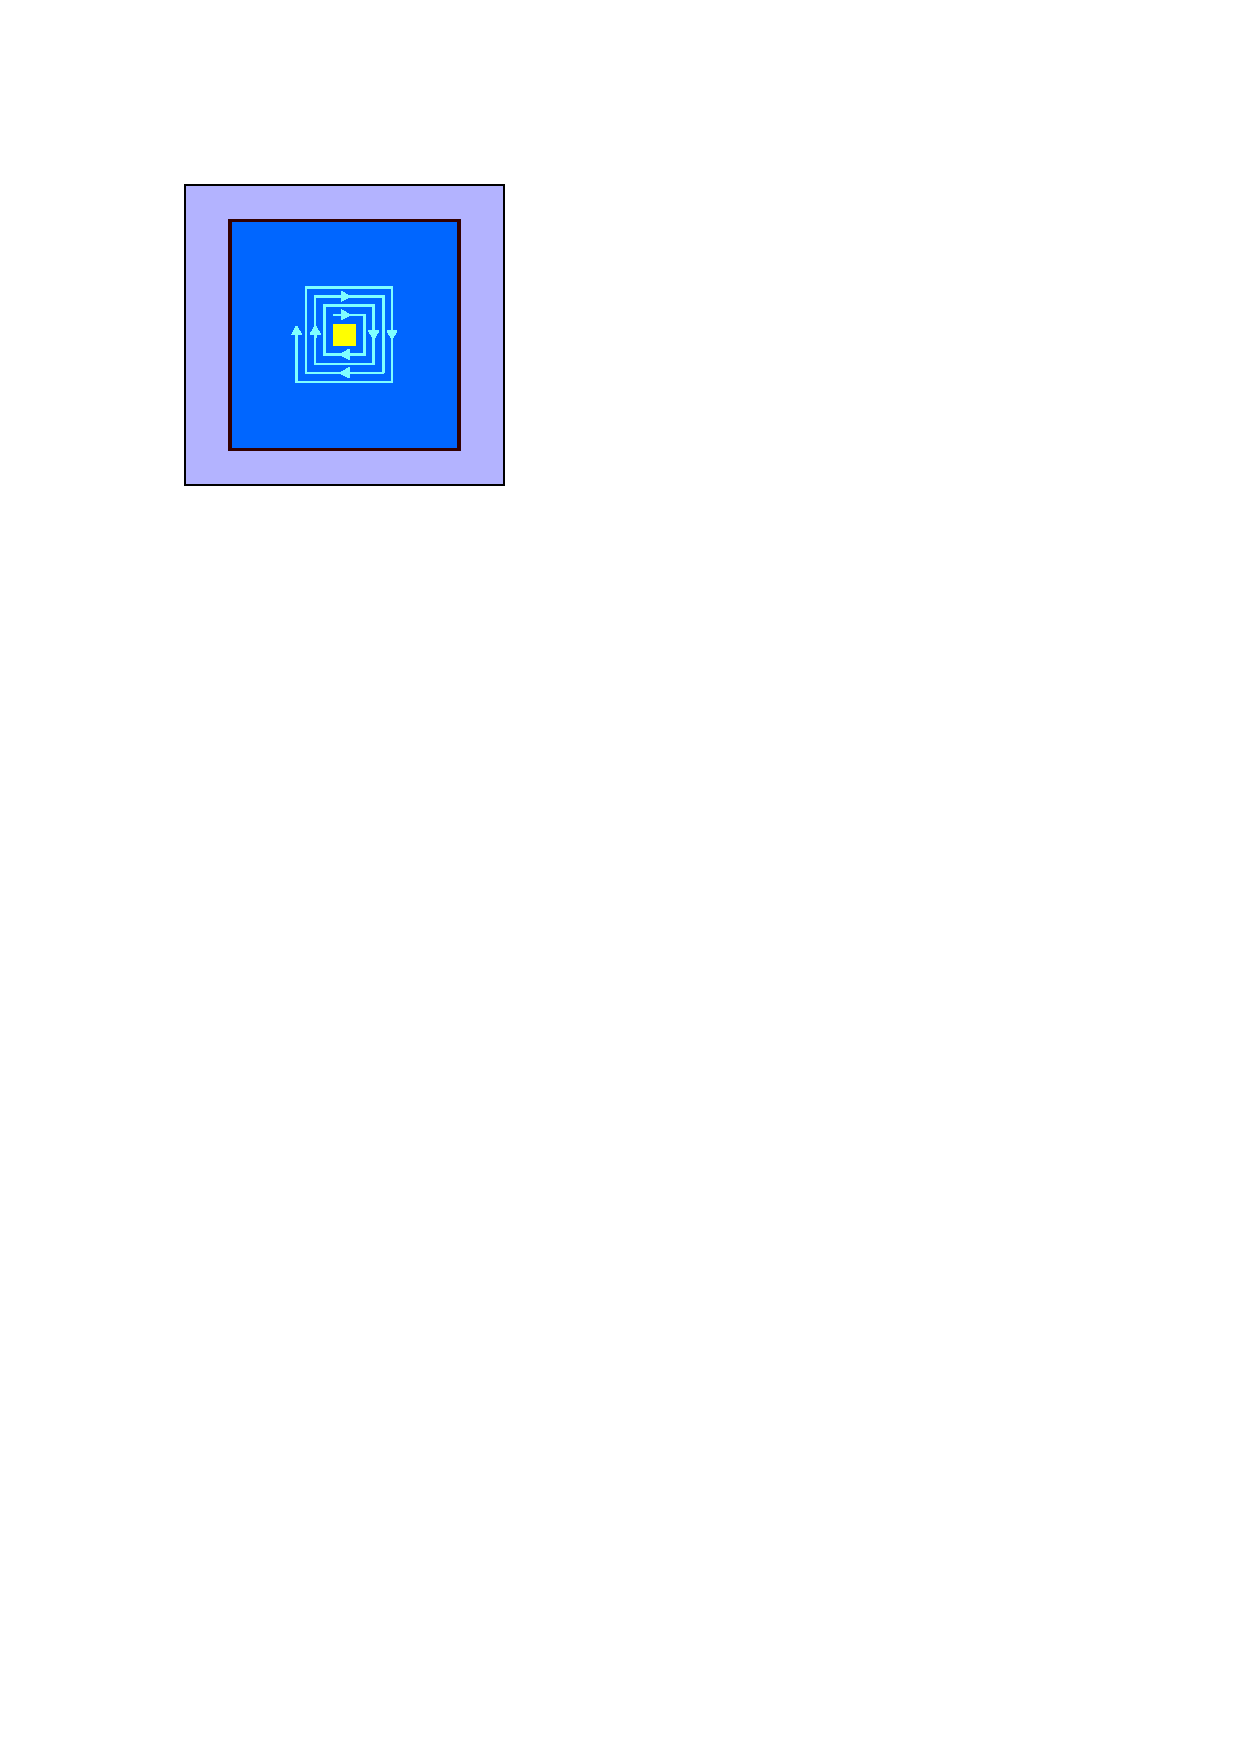
\includegraphics [width=\linewidth]{figures/pixel_keim_spiral.pdf}
    \captionof {figure}{Spiral~\cite{keim94pixel}}
    \label{fig:pixel-spiral}
}
\hfill
\parbox [h]{0.33\textwidth }{
    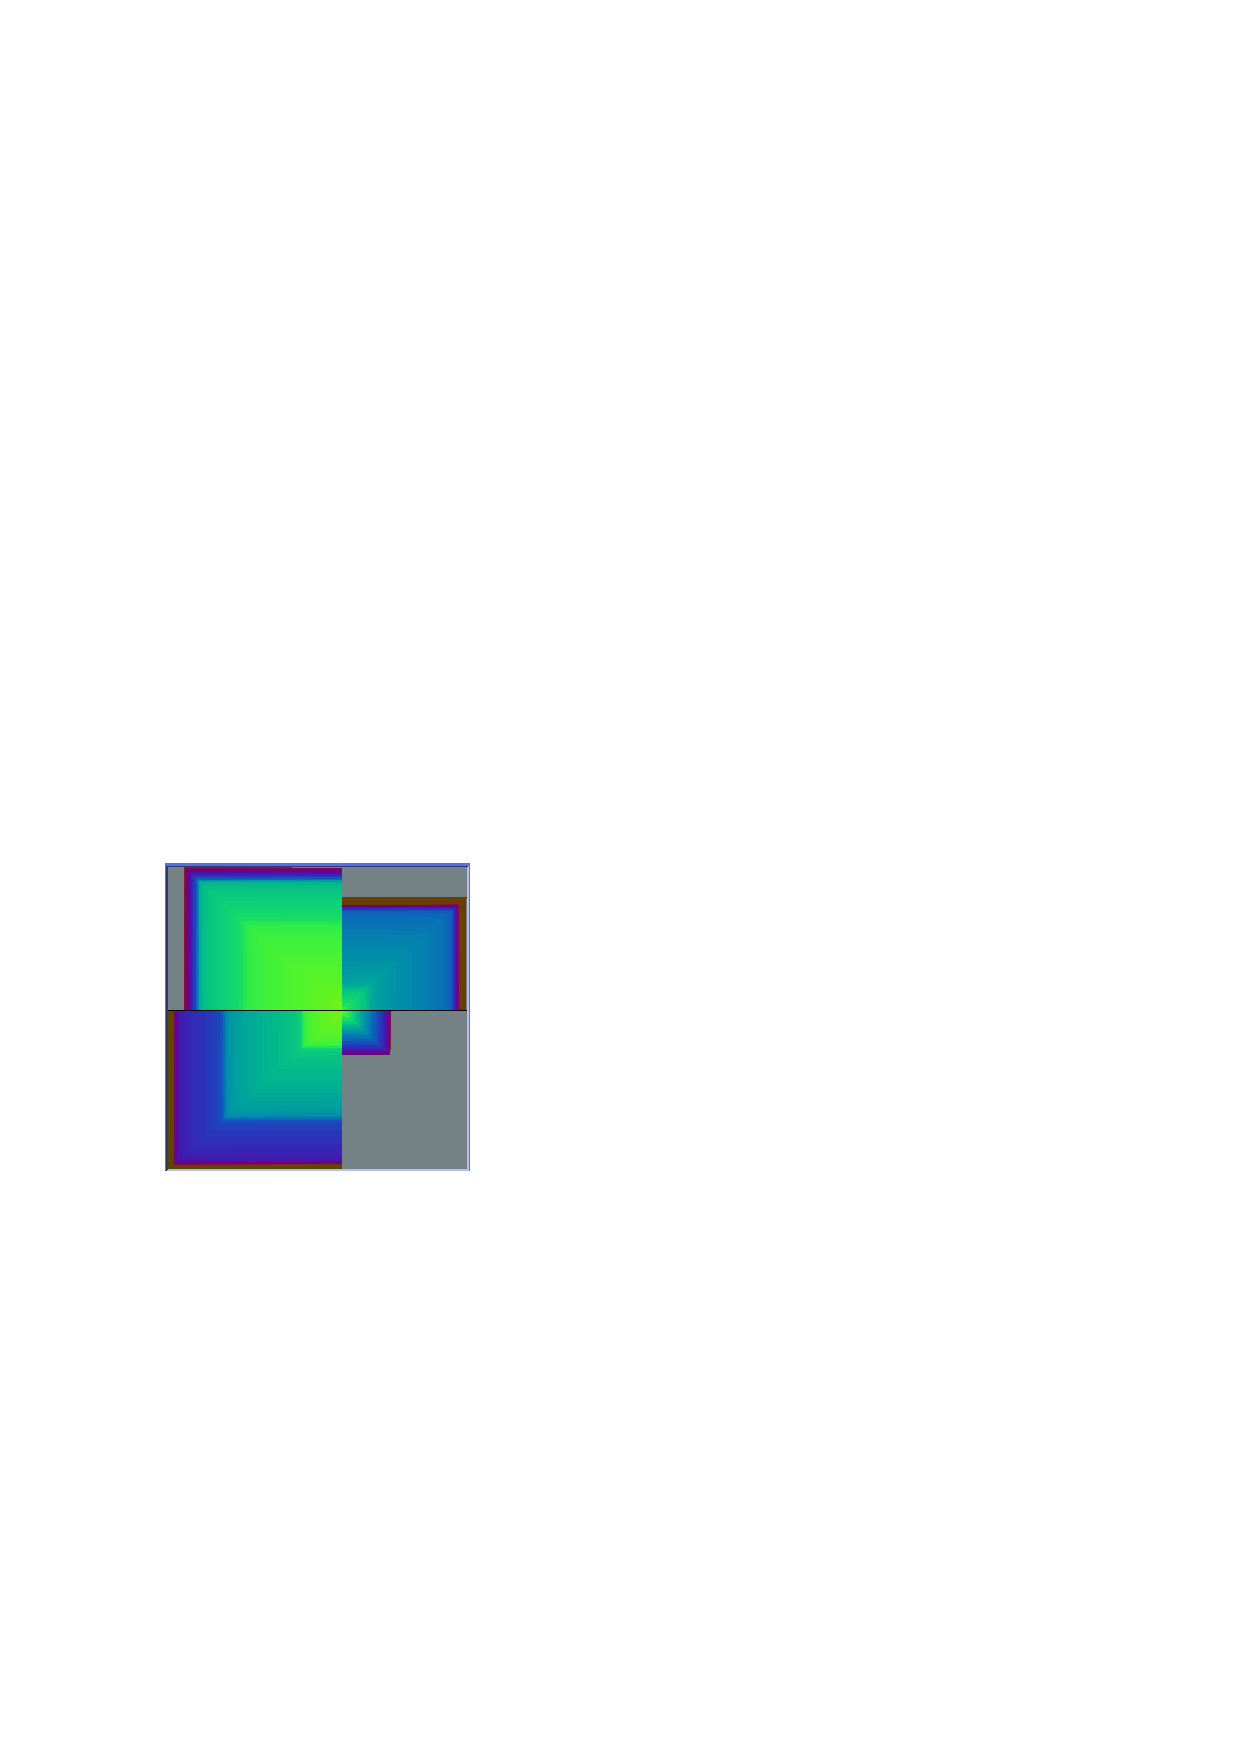
\includegraphics [width=\linewidth]{figures/pixel_keim_axes.pdf}
    \captionof {figure}{Axes \cite{keim94pixel}}
    \label{fig:pixel-axes}
}
\hfill
\parbox [h]{0.35\textwidth }{
    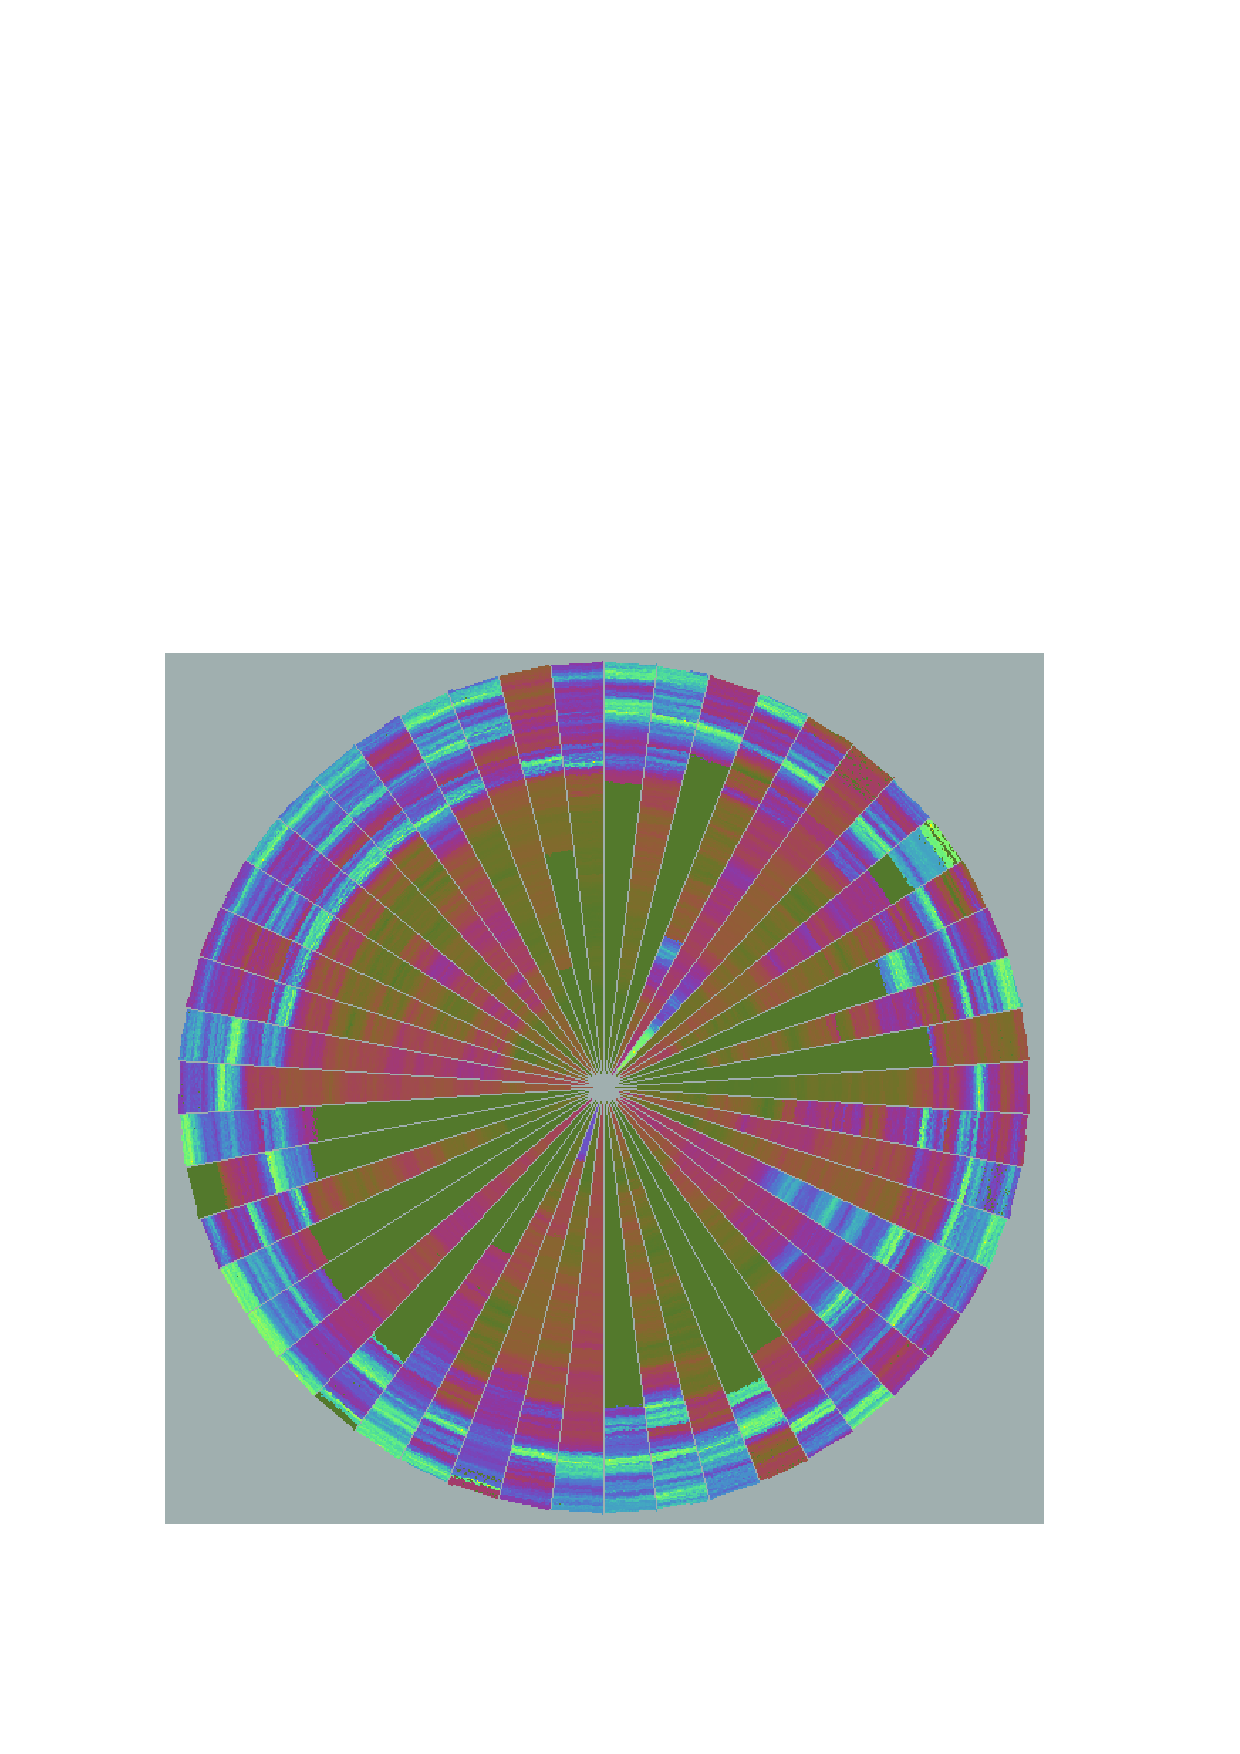
\includegraphics [width=\linewidth]{figures/pixel_keim_circle.pdf}
    \captionof {figure}{Circle \cite{Ankerst96circlesegments}}
    \label{fig:pixel-circle}
}


\item \textbf{Geometric techniques \& Diagrams}

\textit{Geometric techniques} produce useful and insightful visualization by using geometric transformations and projections of the data. \textit{Diagrams} are algorithmically drawn graphics that visualize data. This section lists a selection of geometric techniques for multivariate data presented by Ke-Bing Zhang~\cite{zhang07thesis}, diagram types described by Dieter Ladenhauf~\cite{ladenhauf12dia} and related examples found in additional literature and on the web as stated in the individual references.

\begin{itemize}

\item \textit{Line charts} visualize data as lines by connecting data points of the corresponding values. They are used to display trends over time. Figure \ref{fig:dia-map-sparklines} illustrates surface temperature anomalies from NASA's GISS\footnote{NASA Goddard Institude for Space Studies \url{http://www.giss.nasa.gov/}} as a \textit{Sparkline} map~\cite{web:sparkmaps}. The Sparkline is a reduced line chart without axes and coordinates. It presents the general shape of variation in a simple and highly condensed way~\cite{wiki:sparkline}.

\item \textit{Bar charts} express data values by vertical or horizontal bars, in which the length of a bar indicates the data value. Figure \ref{fig:dia-map-barchart} shows an example from UgandaWatch\footnote{UgandaWatch: \url{http://www.ugandawatch.org/}}, which displays economic indicators per region for the country Uganda. In this example, the Drupal mapping stack explained in chapter \ref{chapter:drupal-mapping} is combined with bar chart technologies\footnote{How are you using mapping in Drupal? \url{http://groups.drupal.org/node/174904\#comment-585264}}.

\parbox [h]{0.4\textwidth }{
    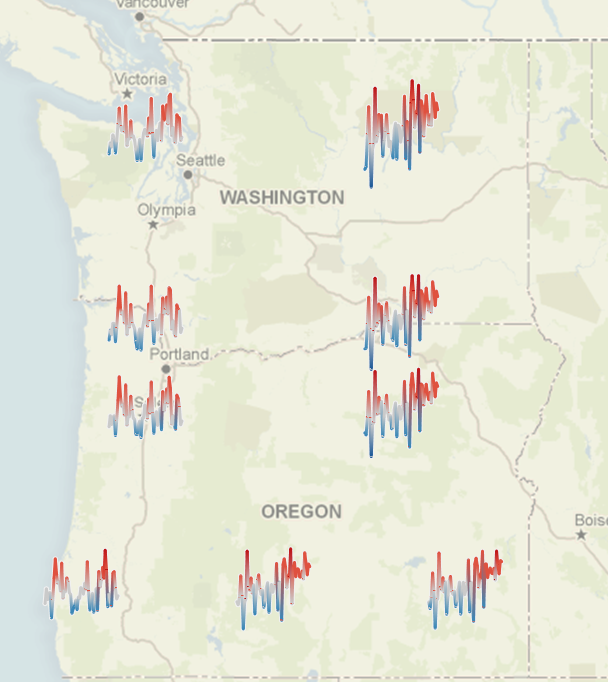
\includegraphics [width=\linewidth]{figures/dia_map_sparklines.png}
    \captionof {figure}{Sparkline map\protect\footnotemark}
    \label{fig:dia-map-sparklines}
}\footnotetext{Sparkline map example: \url{http://www.tableausoftware.com/about/blog/2008/08/sparklines-maps}}
\hfill
\hspace{0.5cm}
\parbox [h]{0.4\textwidth }{
    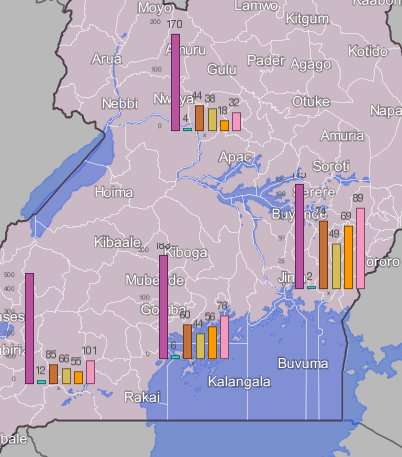
\includegraphics [width=\linewidth]{figures/dia_map_barchart.png}
    \captionof {figure}{Bar chart map\protect\footnotemark}
    \label{fig:dia-map-barchart}
}\footnotetext{UgandaWatch bar chart example: \url{http://www.ugandawatch.org/}}


\item \textit{Pie charts} use a circle divided into sectors for expressing the proportional significance of data values. Variants of pie charts include \textit{doughnut charts}, \textit{three-dimensional pie charts} and \textit{multi-level pie charts}. Also, the \textit{polar area diagram} introduced in figure \ref{fig:map-type-standard-wind} is a special kind of pie chart and a further development of the \textit{Bat's wing diagram} by Florence Nightingale~\cite{night98bart}.

Figure \ref{fig:dia-map-piechart} depicts a pie chart map example from the Kartograph\footnote{Kartograph \url{http://kartograph.org/}} framework. It shows unemployment rates in Spain, providing an effective way to display ratios as opposed to a chloropeth map, where the user usually needs to consult a legend to understand the actual data values.

\item \textit{Container shapes} such as \textit{bounding boxes} and \textit{hulls} are an alternative to iconic displays as they can show the area covered by clusters~\cite{Delort10vis}. As seen in figure \ref{fig:leaflet}, the Leaflet.markercluster library visualizes the convex hull of a cluster to indicate the covered area on mouse-hover. Marco Cristani et al~\cite{Cristani08geoimagemaps} use a hull-based technique for visualizing clusters from a geo-located image database on a map. As illustrated in figure \ref{fig:dia-map-hull}, each cluster is represented by a hull that marks the boundaries of the area and contains a representative image of the clustered set of images.


\parbox [h]{0.4\textwidth }{
    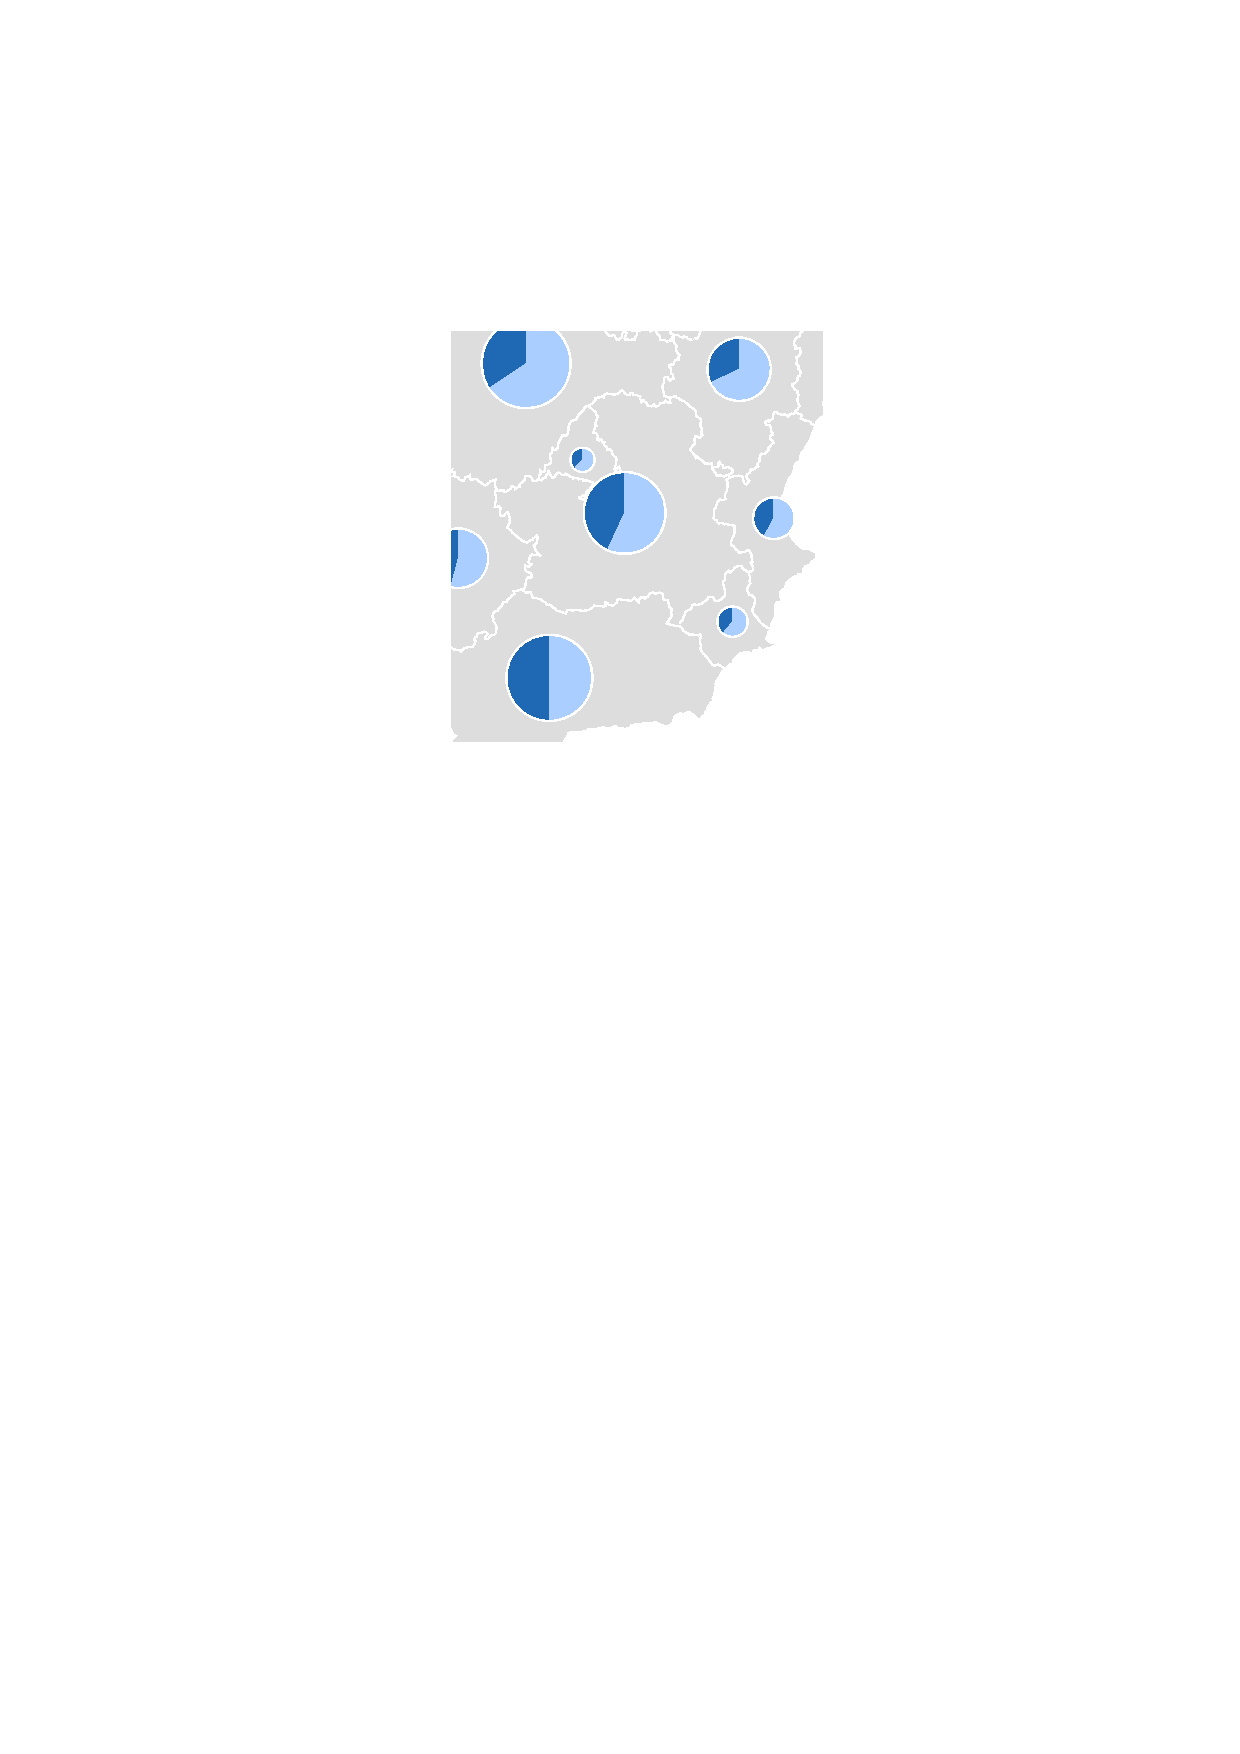
\includegraphics [width=\linewidth]{figures/dia_map_piechart.pdf}
    \captionof {figure}{Pie chart map\protect\footnotemark}
    \label{fig:dia-map-piechart}
}\footnotetext{Pie chart map example from Kartograph: \url{http://kartograph.org/showcase/charts/}}
\hfill
\hspace{0.5cm}
\parbox [h]{0.4\textwidth }{
    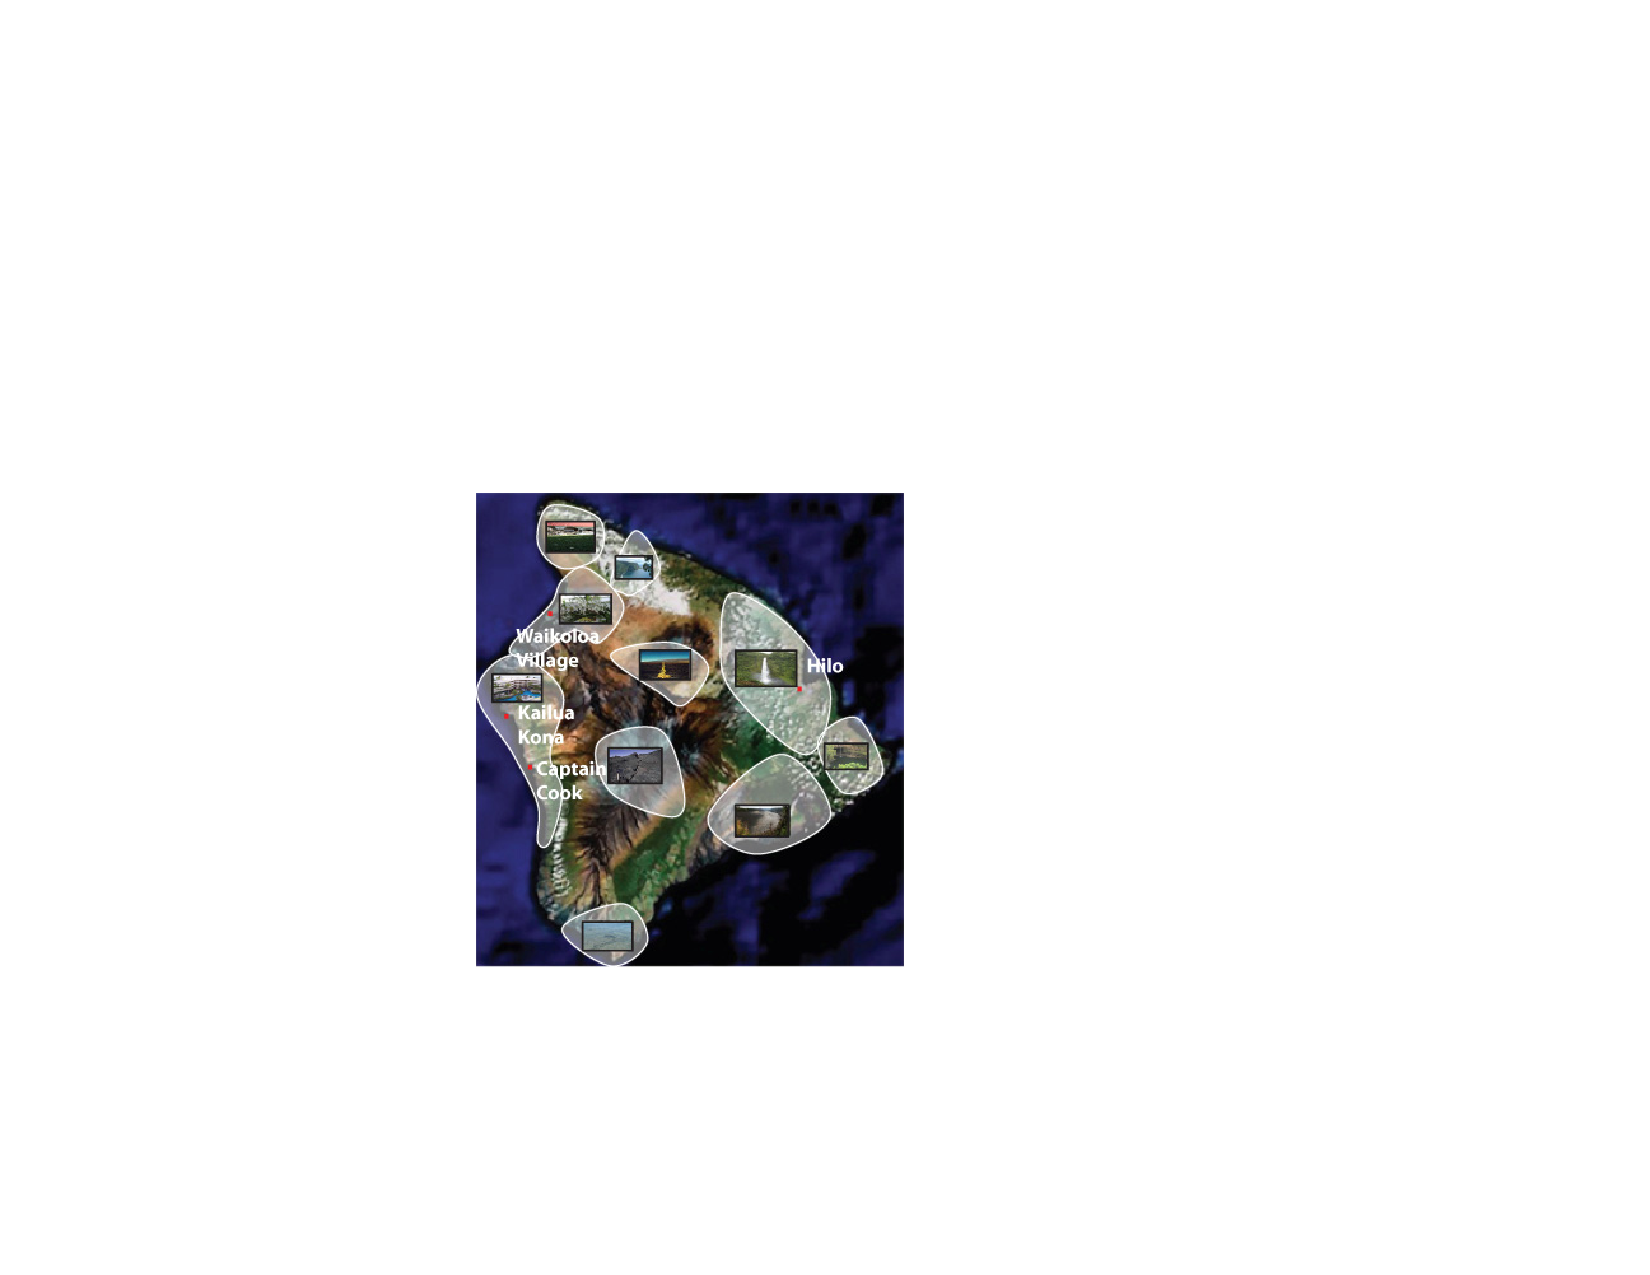
\includegraphics [width=\linewidth]{figures/dia_map_hull.pdf}
    \captionof {figure}{Convex hull map\protect\footnotemark}
    \label{fig:dia-map-hull}
}\footnotetext{Convex hull map example from \cite{Cristani08geoimagemaps}}



\item Further chart types that can possibly used for visualizing clusters on a map include \textit{Area charts} and \textit{Star plots}~\cite{ladenhauf12dia} or more complex ones like \textit{Parallel coordinates}, \textit{Scatterplots}, \textit{Treemaps}~\cite{zhang07thesis} or the \textit{Contingency Wheel++} \cite{VAST2012}. \textit{Bristle maps} are an interesting approach for visualizing spatio-temporal data on a map. Basically, histograms of the data are rendered onto linear map elements. If the data permits a mapping from aggregates to spatial line data, such a visualization technique could be of interest~\cite{bristle}.

\end{itemize}

\end{itemize}

This concludes the investigative enumeration of cluster visualization techniques for maps. It is by no means a complete, but rather an exemplary listing that may provide a starting point when researching visual means of presenting clustered data on a map.

An interesting publication by Andrienko et al~\cite{andrienko2012sca} presents a complex system for place-oriented analysis of movement data. This goes beyond the use case of simply visualizing clustered data on a slippy map, but it is a good show case for how effective the presentation of spatio-temporal data using a combination of techniques can be. \textit{Time graphs}, \textit{mosaic diagrams}, \textit{space-time cubes} and \textit{table lens displays} are used to create a powerful tool for inspecting movement data on maps.

\subsection{Evaluation of visualization techniques for clusters on a map}
\label{chapter:eval-vis}

This chapter summarizes the main visualization examples presented in the previous chapters. An evaluation of techniques for visualizing clusters on maps is created by proposing a set of key characteristics that are considered to be significant for this kind of visualization.

Evaluating information visualization techniques is a well-known problem. Undertaking an evaluation that is capable of ``proving'' the effectiveness is impossible in many situations as it would require too many tasks, data sets, implementations and users. Ellis and Dix state exploratory analysis as the most effective approach for evaluating visualization techniques~\cite{ellis06eval, Delort10vis}. In this sense, the following evaluation should primarily be treated as exploratory and as a help for understanding how cluster visualization on maps works, rather than a final, summative conclusion of which technique is superior than another. 

\textbf{Criteria}. the following, custom criteria have been defined: \textit{category}, \textit{shows number of items within cluster} (\textit{by shape size}, \textit{by color or other}), \textit{shows cluster area}, \textit{shows extra cluster info} \textit{(extra cluster info complexity}). Some criteria contain sub-criteria which are stated within parentheses.

In chapter \ref{chapter:foundations-vis}, three taxonomies have been introduced: \textit{visual variables}, a \textit{classification of visual data exploration techniques} and a \textit{clutter reduction taxonomy}. An attempt to classify the different visualization techniques for representing clusters on maps according to classes introduced by these taxonomies didn't feel valid. Some criteria are too general while others are too specific to actually matter for visualizing clusters on maps, so the resulting data would not have much value. Similarly, a classification based on all \textit{visual variables} would have become very complex. As the presented visualization examples describe general concepts, there are many possible variations that would increase the data set even more. It is still helpful to rely on the aesthetic attributes for a better understanding of how each visualization is constructed. Especially the \textit{shape}, \textit{size} and \textit{color} attributes are considered to have a strong effect on visualizing clusters on maps and are therefore included within the evaluation.

An explanation of each criterion follows:

\begin{itemize}

\item \textbf{category}: Determines the type of visualization technique being evaluated. Possible values are \textit{type of map} (see chapter \ref{chapter:map-vis}), a visualization \textit{example}, as well as abbreviations for cluster visualization techniques (see chapter \ref{chapter:cluster-vis}): \textit{glyph}: Icon-based, Glyphs, \textit{pixel}: Pixel-oriented techniques and \textit{geom}: Geometric techniques \& Diagrams.

\item \textbf{shape}: Defines the type of shape being used for the visualization of clusters on the map. For example \textit{circle} or \textit{area}. Refer to the visual variable shape in chapter \ref{chapter:vis-variables}. 

\item \textbf{shows \# of items within cluster}: If the visualization provides an indicator of the amount of items per clusters. This relates to the `can see overlap density' criterion of the clutter reduction taxonomy, see \ref{clutter-reduction}. Two sub-criteria are used to differentiate between visual means of encoding the number of items within clusters: 

\begin{itemize}

\item \textbf{by shape size}: classifies visualization techniques that use the shape size for indicating the number of items within clusters.

\item \textbf{by color or other}: classifies visualization techniques that use color or other visual indicators to describe the number of items within a cluster.

\end{itemize}

\item \textbf{shows cluster area}: Determines, if the visualization indicates the spatial area that is covered by the cluster or the items within a cluster.

\item \textbf{shows extra cluster info}: Besides the two characteristics of number of items within a cluster and the cluster area, the technique might provide means of visualization additional information of clusters such as aggregates. 

\begin{itemize}

\item \textbf{extra cluster info complexity}: This sub-criterion expands of an intuitive notion of complexity that can be visualized as extra cluster info by the technique. \textit{low} indicates a maximum of three dimensions. \textit{medium} is used to describe up to 12 dimensions of additional data and \textit{high} classifies cluster visualization techniques that go beyond this number of dimensions.

\end{itemize}

\end{itemize}

\begin{figure}[h]
  \begin{center}
    \hspace*{-1.5cm}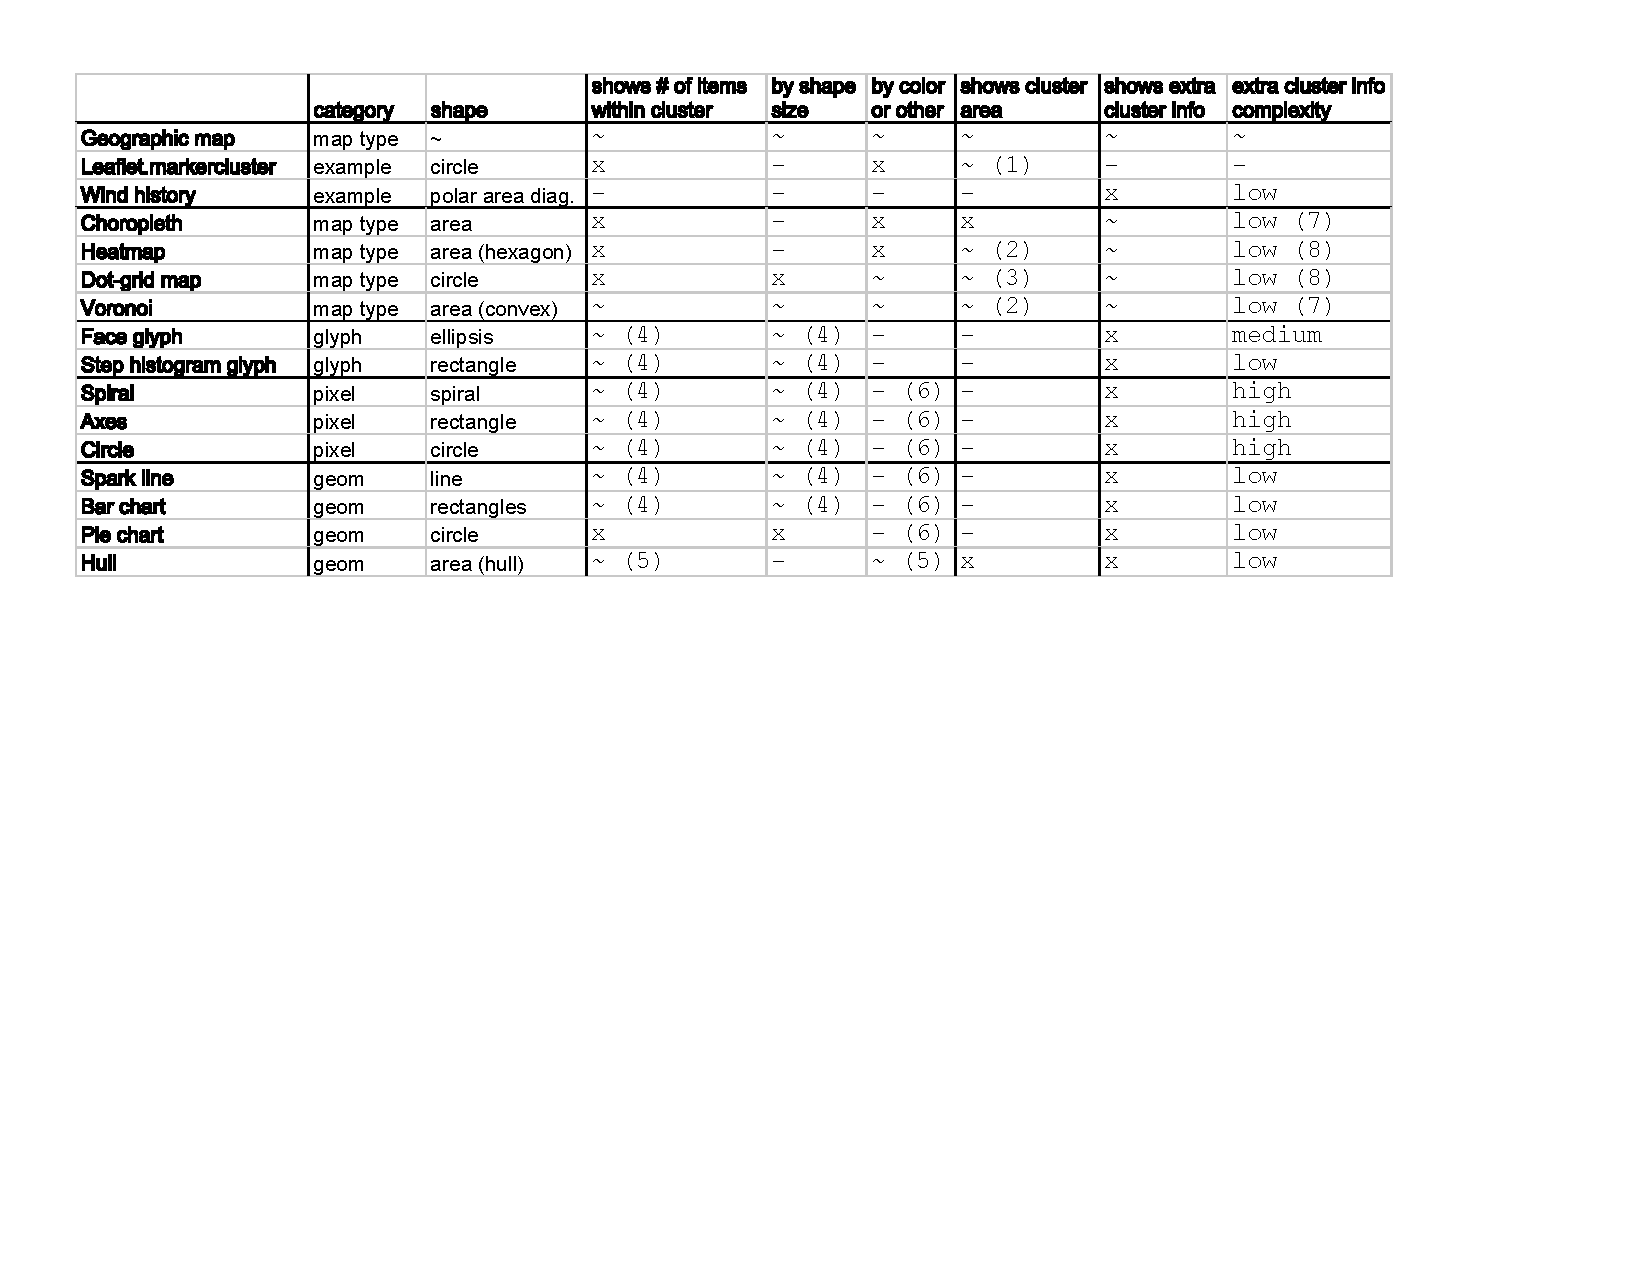
\includegraphics[width=1.2\textwidth]{figures/vis_evaluation.pdf}
    \caption{Evaluation of visualization techniques for clusters on a map. Legend:~`x':~yes,~`\textasciitilde': possibly, `-': no. Numbers in parentheses reference additional notes within the accompanying text.}
    \label{fig:vis-eval}
  \end{center}
\end{figure}

The results of the evaluation of visualization techniques for clusters on a map based on the stated criteria are illustrated in figure \ref{fig:vis-eval}. Note that the classifications for each technique being evaluated primarily represent the according examples shown in the previous chapters. Where it seemed obvious, the optional possibility of fulfilling a criterion has been marked as such. As an extreme example, the geographic map as its general concept has been marked with the optional possibility of fulfilling each criterion. It is up the the actual implementation to satisfy them individually. While the Leaflet.markercluster example provides a visual indicator for the number of items within clusters, the wind history example doesn't.

Some classifications contain a number referring to additional notes as presented in the following: (1) The Leaflet.markercluster example shows cluster on demand, based on user interaction. By mouse-hovering over an item, it will display the convex hull of the items being clustered, see figure \ref{fig:leaflet}. (2) In the case of the binned heat map example and the Voronoi map, cluster areas are approximated by the tessellation which is part of the clustering algorithm, see figure \ref{fig:map-type-binning} and \ref{fig:map-type-voronoi}. (3) The dot-grid map doesn't provide a mean of showing cluster areas by themselves, but the density of items still supports the notion of recognizing cluster areas, see figure{fig:map-type-dotgrid}. (4) For various visualization techniques, the amount of items within a cluster could be visualized by simply scaling the visual entity. (5) The hull example uses an area shape defined by the data, similarly to the choropleth map. Without a distortion technique, the shape therefore can't be used to indicate the number of items within a cluster. Still, a non-shape visual aspect like color could be used as an indicator. (6) In the case of pixel-oriented techniques and the provided chart examples, the color attribute will likely be used for showing extra cluster info instead of indicating the number of items within a cluster. Modifying the shape size can be used as an alternative in this cases. (7) The choroleth and voronoi map examples would rely on representing extra information within the defined area and therefore rely on the.variation of visual variables related to color and texture. (8) The same restrictions as in the previous note apply, but for even smaller areas.

Driving forces in visual mapping, map visualization types and cluster visualization techniques for maps have been introduced and summarized within the given evaluation. This concludes the chapter on state of the art. 

